\chapter{Results}

In thesis I create a port for the HoloLens 2 using the aforementioned Object Tracker. I use Research Mode \cite{ResearchMode} to provide the Object Tracker with the sensor data it needs and create a working application around it which runs on the HoloLens 2. In this chapter I will take a closer look at the indiviual components of my work.

\section{Sensor API}\label{sec:sensorapi}

At the heart of the application lies the Sensor API. It unifies several sensors from different APIs to provide raw data streams. The \lstinline{SensorApi} class serves as the interface between the Sensor API and the application that retrieves its data. It initializes the individual sensor interfaces with their respective APIs and manages them.

Each sensor is represented in the code by a sensor interface. Each sensor interface is running a separate thread in which it continuously loads new data. The \lstinline{SensorApi} class then provides functions for extracting this data by the application processing it. 

In the case of the IMU sensors, \lstinline{SensorApi} only exposes a single function which returns the merged IMU measurements instead of independent measurements for each individual sensor. The measurements from the IMU sensors usually don't arrive at the same time, let alone at the same frame rate. The \lstinline{SensorApi} therefore stores the measurements it receives in separate buffers and returns only complete IMU measurements (consisting of both accelerometer and gyroscope measurements) where data from both sensors has arrived. 

Furthermore the \lstinline{SensorApi} class exposes functions to retrieve extrinsic transformation matrices for all sensors. With these it is possible to create transformation matrices for transformations between any pair of sensors. As mentioned in sec. \ref{sec:ResearchMode}, all sensors are located relative to a rigid node which is determined by Research Mode. For example \lstinline{GetT_gyroscope_rigid()} would return a 4x4 transformation matrix which can be used to transform a vector from the coordinate system of the rigid node into the coordinate system of the gyroscope. For readers unfamiliar with this naming convention, I refer to the appendix sec. \ref{apx:naming}.

The whole Sensor API only uses Mixed Reality Windows APIs and Research mode. The conversion to Eigen, OpenCV and similar libraries used by the Object Tracker is done outside of the Sensor API. It is therefore possible to use this API as a plug and play module which can be integrated into projects with similar use cases.

A UML diagram of all the important classes, properties and methods can be found in fig. \ref{fig:SensorApiUML}. I have implemented interfaces for four different kinds of sensors which I describe briefly in the following subsections.

\begin{empfile}[SensorApiUML]
\begin{empcmds}
input metauml;
\end{empcmds}
\begin{empdef}[SensorApiUML](100,100)
    Class.SensorApi("SensorApi")
           ("-accelData: deque<ImuSensorDataStruct>",
            "-gyroData: deque<ImuSensorDataStruct>") 
            ("+InitializeSensors(): void",
             "+GetImuMeasurements(): deque<ImuMeasurement>",
             "+GetCameraFrame(): CameraFrame",
             "+GetDepthCameraFrame(): DepthCameraFrame",
             "+GetT_rigid_camera(): float4x4",
             "+GetT_accelerometer_rigid: float4x4",
             "+GetT_gyroscope_rigid: float4x4",
             "+GetT_depthCamera_rigid: float4x4");
             
    AbstractClass.ImuInterface("ImuInterface")
            ("#dataBuffer: deque<ImuSensorDataStruct>",
             "#sampleFrequency: int",
             "#updateThread: thread")
            ("+GetBuffer(): deque<ImuSensorDataStruct>",
             "+GetExtrinsics(): float4x4",
             "#GetDirectXExtrinsicsMatrx(): XMFLOAT4X4",
             "#GetSamples(): vector<ImuSensorDataStruct>");
    Class_stereotypes.ImuInterface("<<Research Mode>>");
             
    Class.AccelInterface("AccelInterface")
            ()
            ("#GetDirectXExtrinsicsMatrx(): XMFLOAT4X4",
             "#GetSamples(): vector<ImuSensorDataStruct>");
    Class_stereotypes.AccelInterface("<<Research Mode>>");
             
    Class.GyroInterface("GyroInterface")
            ()
            ("#GetDirectXExtrinsicsMatrx(): XMFLOAT4X4",
             "#GetSamples(): vector<ImuSensorDataStruct>");
    Class_stereotypes.GyroInterface("<<Research Mode>>");
             
    Class.CameraInterface("CameraInterface")
            ("-Trc: float4x4",
             "-lastFrame: CameraFrame")
            ("+GetLastFrame(): CameraFrame",
             "+GetExtrinsics(): float4x4");
             
    Class.DepthCameraInterface("DepthCameraInterface")
            ("-lastFrame: DepthCameraFrame",
             "-updateThread: thread")
            ("+GetLastFrame(): DepthCameraFrame",
             "+GetExtrinsics(): float4x4");
    Class_stereotypes.DepthCameraInterface("<<Research Mode>>");
    
    xPadding:=50;
    yPadding:=70;
    SensorApi.nw = (0,0);
    DepthCameraInterface.nw = atright(SensorApi.ne, xPadding);
    CameraInterface.nw = below(DepthCameraInterface.sw, 20);
    AccelInterface.nw = below(SensorApi.sw, yPadding);
    GyroInterface.nw = atright(AccelInterface.ne, xPadding);
    ImuInterface.nw = below(AccelInterface.sw, yPadding);
    
    drawObjects(SensorApi, ImuInterface, AccelInterface, GyroInterface, CameraInterface, DepthCameraInterface);
    link(aggregationUni)(DepthCameraInterface.w -- atleft(DepthCameraInterface.w, xPadding));
    link(aggregationUni)(CameraInterface.w -- atleft(CameraInterface.w, xPadding));
    link(aggregationUni)(AccelInterface.n -- above(AccelInterface.n, yPadding));
    link(aggregationUni)(GyroInterface.n -- atleft(SensorApi.se, 20));
    link(inheritance)(AccelInterface.s -- ImuInterface.n);
    link(inheritance)(GyroInterface.s -- ImuInterface.ne);
\end{empdef}
\end{empfile}
\begin{figure}
    \centering
    \empuse{SensorApiUML}
    \caption[UML Diagram of the Sensor API]{UML Diagram of the Sensor API: The \lstinline{SensorApi} class manages all sensor interfaces and exposes functions to retrieve data and extrinsic transformation matrices from them. The \lstinline{CameraInterface} class collects its data from Mixed Reality Windows APIs, all other sensor interfaces retrieve their data via Research Mode. \lstinline{ImuInterface} is an abstract class implementing all of the shared code for the sensor interfaces of the different IMU sensors. 
      \label{fig:SensorApiUML}}
\end{figure}

\subsection{Camera Interface}

The \lstinline{CameraInterface} class uses only Mixed Reality Windows APIs to retrive frames of the RGB camera of the HoloLens 2. It retrieves these frames at 30fps with a resolution of 960x540 but the resolution can be configured to be up to 1920x1080. It uses the GUID of the Research Mode rigid node provided by \lstinline{SensorApi} to locate the RGB camera relative to this rigid node. This transformation matrix has the form $T_{RC}$.

The returned \lstinline{CameraFrame} struct looks as follows:

\begin{lstlisting}
struct CameraFrame {
  uint64_t ts;
  SoftwareBitmap bitmap;
  float2 principalPoint;
  float2 focalLength;
  SpatialCoordinateSystem coordinateSystem;
};
\end{lstlisting}

The \lstinline{SoftwareBitmap} class defines all properties of the image, for example data, image width, image height and format. For convenience \lstinline{bitmap} is already converted to BGRA 8-Bit. \lstinline{coordinateSyste} is later used to calculate a transformation between the world coordinate system of the Object Tracker and the world coordinate system of the HoloLens.

\subsection{IMU Interfaces}

The \lstinline{AccelInterface} and \lstinline{GyroInterface} classes represent their respective Research Mode sensors. They share most of their code and therefore inherit it from an abstract super class \lstinline{ImuInterface}. The sensors themselves work at different frame rates and at each frame the Research Mode API returns a buffer of measurement samples. The interfaces then down sample the incoming measurements to a desired frequency, in my case 200 measurements per second. The measurements can than be retrieved as a vector of \lstinline{ImuSensorDataStruct} structs:

\begin{lstlisting}
struct ImuSensorDataStruct {
  uint64_t ts;
  float ImuValues[3];
};
\end{lstlisting}

These measurements are then merged by \lstinline{SensorApi} into \lstinline{ImuMeasurement} structs of the form:

\begin{lstlisting}
struct ImuMeasurement {
  uint64_t ts;
  float AccelValues[3];
  float GyroValues[3];
};
\end{lstlisting}

Extrinsic transformation matrices are retrieved directly from research mode and take the form $T_{AR}$ and $T_{GR}$ respectively.

While I didn't implement a sensor interface for the magnetometer since it is not needed for the Object Tracker, it should be trivial to do so since its Research Mode sensor shares most of its behaviour with the other IMU sensors.

\subsection{Depth Camera Interface}

As mentiond in sec. \ref{sec:holHardware}, \lstinline{DepthCameraInterface} has two possible modes of operation, AHAT or Long Throw. Which one to use is defined by \lstinline{SensorApi}. Independent of the mode, the interface can be queried  for the \lstinline{DepthCameraFrame} struct: 

\begin{lstlisting}
struct DepthCameraFrame {
  uint64_t ts;
  uint32_t width;
  uint32_t height;
  std::vector<uint16_t> depthData;
  std::vector<uint16_t> activeBrightnessImage;
};
\end{lstlisting}

Here \lstinline{depthData} is a vector of size \lstinline{width * height} containing the depth values for each pixel. Invalid pixels contain a value of 0. \lstinline{activeBrightnessImage} is a vector of the same size and contains the original infrared image used to calculate the depth map.

At the moment, this sensor is not used by the Object Tracker algorithm and therefore disabled in \lstinline{SensorApi}. However it is ready to be used at either a later point in time or by a different application.

\section{Object Tracker Integration}\label{sec:objectTrackerIntegration}

I now use the Sensor API to retrieve the raw sensor data and feed it into the Object Tracker. The main interface for the Object Tracker is the \lstinline{ObjectTracker} class which exposes various functions to interact with the library. To connect the \lstinline{ObjectTracker} and \lstinline{SensorApi} classes I have created the \lstinline{ViotApplication} class. This class first initiates an instance of \lstinline{SensorApi} and then waits for all sensors to be initialized and ready. Once that is the case, it initializes the \lstinline{ObjectTracker} by loading a configuration file. This file allows for the specification of various configurations such as brick size, which building plan to use and if a log file should be created.

Next the $T_{CameraIMU}$ transformation matrix needs to be set so the \lstinline{ObjectTracker} can transform IMU measurements to the camera space and vice-versa. Since the object tracker doesn't distinguish between different IMU sensors but treats them as a single sensor, we choose to define the IMU position as the position of the accelerometer. To calculate $T_{CameraIMU}$, we retrieve $T_{RigCamera}$ and $T_{AccelRig}$ from the Sensor API and set:

\begin{equation*}
    T_{CameraIMU} := T_{RigCamera}^{-1} * T_{AccelRig}^{-1}
\end{equation*}

The camera calibration also needs to be set in the \lstinline{ObjectTracker}. These parameters can be read directly from the current \lstinline{CameraFrame} provided by \lstinline{SensorApi}.

\lstinline{ViotApplication} runs a separate thread for the RGB camera, the depth camera and the IMU sensor each. Again, the depth camera thread is disabled because it is not needed at the current time. Whenever new data arrives, it is retrieved from the \lstinline{SensorApi} instance, transformed into the format \lstinline{ObjectTracker} expects, and fed into it. For example are IMU measurements converted to Eigen vectors and images are converted to OpenCV matrices. This process is shown in fig. \ref{fig:dataThreads}.

\begin{figure}
    \centering  
    \begin{sequencediagram}
        \newthread{ViotThread}{ViotApplication::SensorThread}
        \newinst{SensorApi}{SensorApi}
        \newinst{SensorInterface}{SensorInterface}
        \newthread{SensorThread}{SensorInterface::DataThread}
        
        \begin{call}{SensorThread}{WaitForData()}{SensorThread}{}
        \end{call}
        \begin{call}{SensorThread}{SaveData()}{SensorInterface}{}
        \end{call}
        \mess{SensorThread}{notify}{ViotThread}
        \begin{call}{ViotThread}{GetData()}{SensorApi}{return data}
            \begin{call}{SensorApi}{GetData()}{SensorInterface}{return data}
            \end{call}
        \end{call}
        \begin{call}{ViotThread}{AddToObjectTracker(data)}{ViotThread}{}
        \end{call}
        \begin{call}{SensorThread}{WaitForData()}{SensorThread}{}
        \end{call}
    \end{sequencediagram}
    \caption[Abstracted sequence diagram of data thread interactions]{Abstracted sequence diagram of data thread interactions: Each sensor interface runs a thread to continuously fetch data from its sensor which is then saved in the sensor interface instance. After that, the respective thread of the \lstinline{ViotApplication} instance is notified which then retrieves the data from the sensor interface via the \lstinline{SensorApi} and feeds it into the \lstinline{ObjectTracker}. \lstinline{ViotApplication} runs one thread for each sensor type.}
    \label{fig:dataThreads}
\end{figure}

Since the position of the accelerometer is treated as the IMU position, gyroscope measurements need to be transformed into the accelerometer space. For this the rotation matrices $R_{AccelRig}$ and $R_{GyroRig}$ are extracted from $T_{AccelRig}$ and $T_{GyroRig}$ respectively which are retrieved from the \lstinline{SensorApi}. All gyroscope measurements are then rotated by:

\begin{equation*}
    R_{AccelGyro} = R_{AccelRig} * R_{GyroRig}^{-1}
\end{equation*}

It is not necessary to perform use the full transformation matrix (i.e. include the translation) because gyroscope measurements are translation invariant.

Because IMU measurements can lag behind camera frames by up to 0.3 seconds, camera frames are stored in a buffer and only fed into the \lstinline{ObjectTracker} when the corresponding IMU measurements have arrived. This way \lstinline{ObjectTracker} doesn't wait idly for IMU measurements to arrive but optimizes the last available state. 

After feeding camera frames into the \lstinline{ObjectTracker}, \lstinline{ViotApplication} retrieves the latest estimation for $T_{WorldIMU}$ by the \lstinline{ObjectTracker}. The pose of the camera at the same time is then used to calculate the estimated transformation matrix from the HoloLens world to the Object Tracker world. This is necessary to be able to transform objects from the world coordinate system of the Object Tracker in which they are tracked into the world coordinate system of the HoloLens in which they are drawn.

The user interface thread of the application calls the \lstinline{Update()} and \lstinline{Draw()} functions of \lstinline{ViotApplication} once every iteration. During \lstinline{Update()} the poses of all objects are updated with the estimates provided by the \lstinline{ObjectTracker} while \lstinline{Draw()} draws them into the holographic space.

An UML diagram of the this part of the application can be seen in fig. \ref{fig:ObjectTrackerUML}.

\begin{empfile}[ObjectTrackerUML]
\begin{empcmds}
input metauml;
\end{empcmds}
\begin{empdef}[ObjectTrackerUML](100,100)
    Class.SensorApi("SensorApi")
           () 
            ("+GetImuMeasurements(): deque<ImuMeasurement>",
             "+GetCameraFrame(): CameraFrame",
             "+GetDepthCameraFrame(): DepthCameraFrame",
             "+GetT_rigid_camera(): float4x4",
             "+GetT_accelerometer_rigid: float4x4",
             "+GetT_gyroscope_rigid: float4x4",
             "+GetT_depthCamera_rigid: float4x4");
             
    Class.ViotApplication("ViotApplication")
            ("-imuThread: thread",
             "-cameraThread: thread",
             "-depthThread: thread",
             "-cameraBuffer: deque",
             "-drawDebugImage: bool")
            ("+StartPoseInitialization(): void",
             "+EndPoseInitialization(): void",
             "+RequestStep(): void",
             "+RequestStepBack(): void",
             "+StopTracking(): void",
             "+ToggleFullPlan(): void",
             "+GetTrackerState(): TrackerState",
             "+Update(): void",
             "+Draw(): void");
            
    Class.ObjectTracker("ObjectTracker")
            ()
            ("+addImuMeasurement(ts:double, accel:Vector3, gyro:Vector3): void",
             "+addImage(ts:double, image:Mat): void",
             "+setTciExternally(Tci:Pose): void()",
             "+setCameraCalibration(focal:float2, principal:float2, height:int, width:int): void",
             "+state(): TrackerState",
             "+startPoseInit(): void",
             "+donePoseInit(): void",
             "+stepRequest(): void",
             "+stepBackRequest(): void",
             "+stopTrackingRequest(): void",
             "+setVisualizFullBuildingPlan(show:bool): void",
             "+GetPendingObjectPose(): Pose",
             "+GetMostRecentObjectPoses(): vector<Pose>",
             "+getLatestTwiEstimate(Twi:Pose, ts:double): void");
    
    topToBottom(70)(SensorApi, ViotApplication, ObjectTracker);
    
    drawObjects(ViotApplication, SensorApi, ObjectTracker);
    
    link(aggregationUni)(SensorApi.s -- ViotApplication.n);
    link(aggregationUni)(ObjectTracker.n -- ViotApplication.s);
\end{empdef}
\end{empfile}
\begin{figure}
    \centering
    \empuse{ObjectTrackerUML}
    \caption[UML Diagram of the Object Tracker integration]{UML Diagram of the Object Tracker integration: The \lstinline{ViotApplication} class retrieves data from the \lstinline{SensorApi}, transforms it into the correct format and feeds it into the \lstinline{ObjectTracker}. It is also responsible for updating and drawing tracked objects retrieved from \lstinline{ObjectTracker}.
      \label{fig:ObjectTrackerUML}}
\end{figure}

\subsection{User Interface}

The user interface consists of five buttons which are either enabled or disabled depending on the current state of the Object Tracker. The Object Tracker can be in one of three states:

\begin{itemize}
    \item HOLD: The Object Tracker is idle and waits for tracking to start.
    \item INIT: The Object Tracker is in the process of being initialized. In this state the user can place the first brick and start tracking when he or she is finished.
    \item TRACKING: The Object Tracker is in the process of tracking. 
\end{itemize}

The five buttons are:

\begin{itemize}
    \item Start Init: This button starts the pose initialization of the Object Tracker. This means, the first brick will be drawn and move with the users head.
    \item Done Init: Once the brick moving with the users head is correctly positioned, this button may be pressed to lock it in place. This starts the tracking of the brick.
    \item Next: This button goes one step forward. This means that if all active objects have been placed, a new pending object is added and if a pending object is ready to be tracked, it changes this object's state from pending to active. 
    \item Back: This button does the reverse of the Next button.
    \item Stop: This button stops the tracking.
\end{itemize}

The state of each button depending on the state of the Object Tracker can be found in tab. \ref{tab:buttonStates}.

\begin{table}
\centering
\begin{tabular}{ | l | c | c | c | c | c | }
 \hline
 & \textbf{Start Init} & \textbf{Done Init} & \textbf{Next} & \textbf{Back} & \textbf{Stop} \\
 \hline
 \textbf{HOLD} & \checkmark & \text{\sffamily X} & \text{\sffamily X} & \text{\sffamily X} & \text{\sffamily X} \\
 \textbf{INIT} & \text{\sffamily X} & \checkmark & \text{\sffamily X} & \text{\sffamily X} & \checkmark \\
 \textbf{TRACKING} & \text{\sffamily X} & \text{\sffamily X} & \checkmark & \checkmark & \checkmark \\
 \hline
\end{tabular}
\caption[Active UI buttons depending on the Object Tracker state]{The state of each button of the user interface depending on the current state of the Object Tracker. A checkmark means that the button is enabled in this state, while an \text{\sffamily X} means it is disabled.}
\label{tab:buttonStates}
\end{table}

The buttons are placed in a row on the lower part of the users viewport. A screenshot can be seen in fig. \ref{fig:ui}. The state transitions in the object tracker triggered by the buttons can be seen in fig. \ref{fig:ObjectTrackerStates}.

\begin{figure}
    \centering
    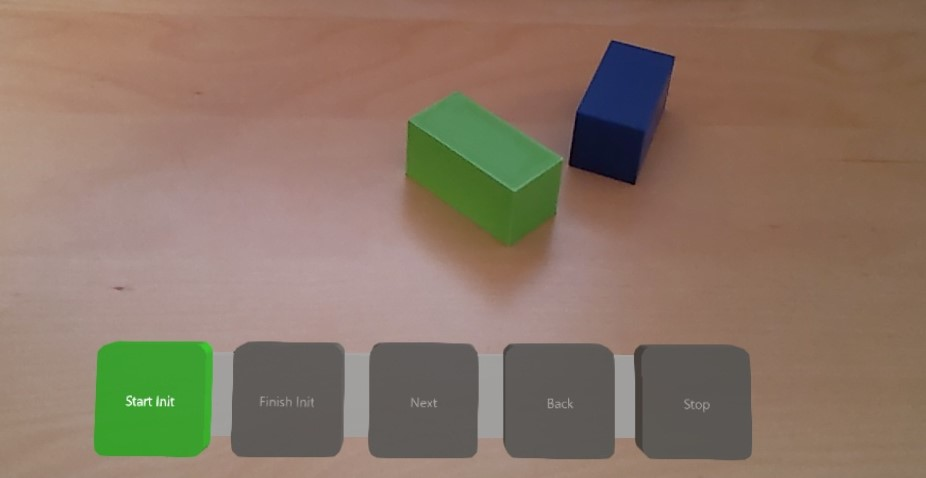
\includegraphics[width=0.9\linewidth]{figures/hololens_ui.jpg}
    \caption[Screenshot of the user interface]{Screenshot of the user interface: The buttons are lined up on the bottom half of the viewport and enabled or disabled depending on the state of the object tracker. In this case, only the first button is enabled.}
      \label{fig:ui}
\end{figure}

\begin{empfile}[ObjectTrackerStates]
\begin{empcmds}
input metauml;
\end{empcmds}
\begin{empdef}[ObjectTrackerStates](100,100)
    State.Hold("HOLD")();
    State.Init("INIT")();
    State.Tracking("TRACKING")();
    
    boxit.Start("StartInit");
    boxit.Done("DoneInit");
    boxit.Next("Next");
    boxit.Back("Back");
    boxit.Stop1("Stop");
    boxit.Stop2("Stop");
    
    leftToRight(70)(Hold, Init, Tracking);
    
    Start.s = above(atright(Hold.e, 35), 5);
    Done.s = above(atright(Init.e, 35), 5);
    Stop1.s = above(Init.n, 25);
    Stop2.n = below(atright(Hold.se, 35), 25);
    Next.n = below(Tracking.s, 30);
    Back.n = below(Tracking.s, 40);
    
    drawObjects(Hold, Init, Tracking);
    drawunboxed(Start, Done, Next, Back, Stop1, Stop2);
    link(transition)(Hold.e -- Init.w);
    link(transition)(Init.e -- Tracking.w);
    link(transition)(pathCut(Tracking, Hold)(Tracking.n -- above(Tracking.n, 20) -- above(Hold.n, 20) -- Hold.n));
    link(transition)(pathCut(Init, Hold)(Init.s -- below(Init.s, 20) -- below(Hold.s, 20) -- Hold.s));
    link(transition)(atleft(Tracking.s, 5) .. below(Tracking.s, 30) .. atright(Tracking.s, 5));
\end{empdef}
\end{empfile}
\begin{figure}
    \centering
    \empuse{ObjectTrackerStates}
    \caption[State transition diagram for the object tracker UI]{State transition diagram for the object tracker UI: Boxes represent the possible states the object tracker can be in while transitions represent button presses in the user interface.
      \label{fig:ObjectTrackerStates}}
\end{figure}

When a brick is not positioned correctly the Object Tracker provides poses for arrows which are then drawn at the corners of the brick. This helps the user to correct the position.

\subsection{Debug Screen}

\begin{figure}
    \centering
    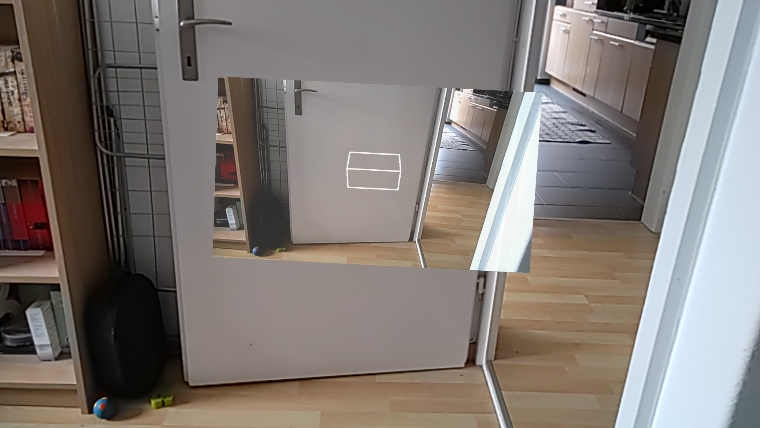
\includegraphics[width=0.9\linewidth]{figures/debug_screen.jpg}
    \caption[Debug Screen for Development]{This image shows the debug screen which can be enabled in \lstinline{ViotApplication} debugging and easier development}
      \label{fig:debugScreen}
\end{figure}

To help with development and debugging, I also provide a debug screen which can be enabled in \lstinline{ViotApplication}. It draws a virtual screen which moves with the user's head and can display any image required. It is especially useful for showing what the Object Tracker would render but it can be configured to show any other image stream.

\subsection{Showcase}

\begin{figure}
    \centering
    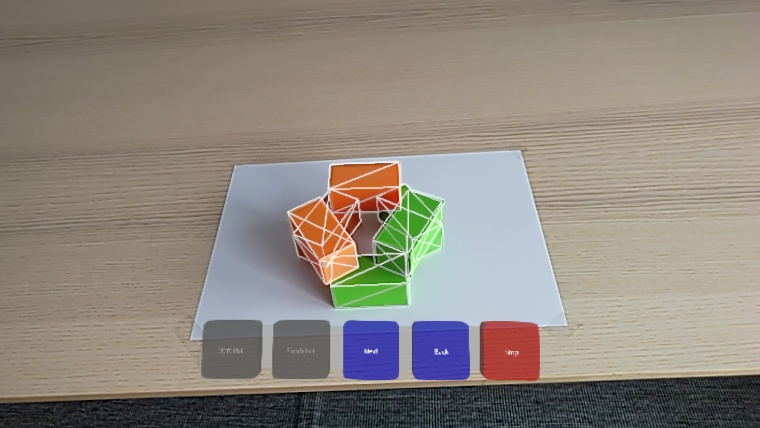
\includegraphics[width=0.9\linewidth]{figures/teaser.jpg}
    \caption[Showcase]{Brick tower built with the Object Tracker on the HoloLens 2. The image shows a screenshot of the HoloLens 2.}
      \label{fig:showcase}
\end{figure}

Fig. \ref{fig:showcase} shows a brick tower built with application presented in this thesis. A video of the complete build process is linked in appendix sec. \ref{apx:video}.

\section{Limitations}

As already mentioned in sec. \ref{sec:objectTrackerIntegration} the IMU measurements provided by Research Mode generally lag up to 0.3 seconds behind the camera frame. Because of this, camera frames have to be held back until the corresponding IMU measurements have arrived. This, of course leads to noticeable delays in the information retrieved from the Object Tracker. Furthermore, while it is possible to use large numbers of IMU measurements per second (I use 200 for this application but larger numbers are possible), these measurements arrive in large batches but at a low frame rate of between 12Hz to 22Hz which leads to the input of a lot of measurements simultaneously. It would be preferred to provide these measurements in a more continuous stream.

The most noticeable limitation imposed by the delayed IMU measurements occurs during the initialisation of the first object pose. It is decidedly more challenging because the pose which should move with the head of the user has a noticeable delay. Once the first pose is initialized it gets better but from time to time one can still notice delayed readjustments of the brick poses to head movement. 

Another limitation is the computing power of the HoloLens 2 in general. Because of this, the Object Tracker often needs longer to optimize than it would on a modern phone. This can lead to even more delayed adjustments, general instability or even loss of tracking.